\documentclass[14pt,a4paper]{ctexbook}

% choose options for [] as required from the list
% in the Reference Guide, Sect. 2.2
\usepackage{indentfirst}
\usepackage{fancyhdr}
\usepackage{longtable}
\usepackage{makeidx}
\usepackage{hhline}
\usepackage{mathpazo}
\usepackage[svgnames]{xcolor}
\usepackage{pifont}
\usepackage{graphicx}        % standard LaTeX graphics tool
\usepackage{float}  % force the figure at specified location
\usepackage{multirow}
\usepackage{geometry}
\usepackage{diagbox}
\usepackage{amsmath}
\usepackage{amssymb}
\usepackage{longtable}
\usepackage{threeparttable}% tables with footnotes
\usepackage{subfigure}
\usepackage{enumitem}
\usepackage{subfigmat}% matrices of similar subfigures, aka small mulitples
\usepackage{nomencl}
\usepackage{lscape}
\usepackage[hyphens]{url}
\usepackage[colorlinks=true, linkcolor=Blue, urlcolor=Maroon,citecolor=red]{hyperref}

\usepackage[sorting=none,style=numeric,backend=biber]{biblatex}
\usepackage{titlesec}

%% set double Chinese characters
\par\setlength\parindent{2em}

% define a new list with no indent for itemed text
\newlist{dingautolist2}{enumerate}{1}
\setlist[dingautolist2,1]{
  labelindent=\parindent,
  leftmargin=\parindent,
  listparindent=\parindent,
%  labelwidth=2pt,
%  itemsep=2pt,
%  label=(\alph*),
%  label=\protect\circled{\arabic*},
%  label=\protect\textcircled{\small\arabic*},
  label=\protect{\protect\ding{\value*}},
  start=192,
  align=left,
  itemsep=0pt,
  wide=\parindent,
  itemindent=\parindent
%  itemindent=\dimexpr\parindent+\labelwidth+\labelsep\relax
}

%makeindex sample.nlo -s nomencl.ist -o sample.nls
\makeindex

% run gbk2uni *.out file between two runs of latex *.tex

% used for the subject index
% please use the style sprmidx.sty with
% your makeindex program
%%%%%%%%%%%%%%%%%%%%%%%%%%%%%%%%%%%%%%%%%%%%%%%%%%%%%%%%%%%%%%%%%%%
\graphicspath{{./eps/}}
\addbibresource{economics.bib}

%% rename the figure/table to 图/表
\renewcommand{\figurename}{图}
\renewcommand{\tablename}{表}
\renewcommand{\contentsname}{目录}
\renewcommand*\listfigurename{图例}
\renewcommand*\listtablename{表例}
\renewcommand{\bibname}{参考文献}

%%% set headers 
\pagestyle{fancy}
\lhead{Aviation Economics}
\rhead{\thepage}
\cfoot{Shanghai Jiao Tong University}
\renewcommand{\headrulewidth}{0.4pt}
\renewcommand{\footrulewidth}{0.4pt}

% Subtract 1 from counters that are used
\renewcommand{\thesection}{\thechapter.\number\numexpr\value{section}\relax}
\renewcommand{\thesubsection}{\thesection.\number\numexpr\value{subsection}\relax}
\renewcommand{\thesubsubsection}{\thesubsection.\number\numexpr\value{subsubsection}\relax}
\setcounter{secnumdepth}{3}

\setcounter{chapter}{0}% Not using chapters, but they're used in the counters

\renewcommand{\chaptername}{章}
\renewcommand{\figurename}{图}
\renewcommand{\tablename}{表}
\renewcommand{\contentsname}{目录}
\renewcommand*\listfigurename{图例}
\renewcommand*\listtablename{表例}
\renewcommand{\bibname}{参考文献}

%%% change the format of chapter
\renewcommand\thechapter{\arabic{chapter}}
\titleformat{\chapter}{\centering\Large\bfseries}{第\,\thechapter\,章}{1em}{}

%%% change the format of subsubsection
\renewcommand\thesubsubsection{\arabic{subsection}}

%%% change the format of subsubsection
\renewcommand\thesubsubsection{\arabic{subsubsection}}
\titleformat{\subsubsection}[block]{\sffamily}{\arabic{subsubsection})}{1em}{}



\begin{document}

\pagenumbering{arabic} % change to arabic
\setcounter{secnumdepth}{3} 
\setlength{\parindent}{2em}
\setlength\intextsep{1.25\baselineskip plus 2pt minus 4pt}


%% first line indentation
%\let\@afterindentfalse\@afterindenttrue
%\@afterindenttrue

\begin{titlepage}
\newcommand{\HRule}{\rule{\linewidth}{0.1mm}} 
\center % Center everything on the page
 
%---------------------------------------------------------------------------------
%     HEADING SECTIONS (Enter the Homework/assignment No., only)
%---------------------------------------------------------------------------------
\textsc{\Large 上海交通大学}\\[0.5cm] % heading course Number
\textsc{\Large 航空航天学院}\\[0.5cm] % heading course name

%---------------------------------------------------------------------------------
%     TITLE SECTION (Replace 'TITLE' with the Homework/assignment Name/title)
%---------------------------------------------------------------------------------
 
\HRule \\[0.4cm]
{ \huge \bfseries Aviation Economics}\\[0.1cm] % Title of your Homework/assignment
\HRule \\[1.5cm]
 
%---------------------------------------------------------------------------------
%     AUTHOR SECTION (EDIT THE NAME and T.NO., only)
%---------------------------------------------------------------------------------
 
\begin{minipage}{0.4\textwidth}

\begin{center}
    \centering
\emph{Song Wenbin} 著 \\
\end{center}\large 

\end{minipage}\\[5cm]

\vspace*{\fill}  % place text at the end of page 
{

\includegraphics[width=0.6\textwidth]{sjtu-logo.eps} \\[1cm]
\large \today}\\[1cm] % Date, change the \today to a set date if you want to be precise
\vfill % Fill the rest of the page with white-space
\end{titlepage}
\include{GradingRubric}

\tableofcontents          % Required
\listoffigures
\listoftables
\newpage

%%%%%%%%%%%%%%%%
\title{Aviation Economics}
\author{Song Wenbin}

\date
\maketitle

\newpage
\makenomenclature
%\pdfbookmark[1]{Contents}{table}

\chapter*{Introduction}
\addcontentsline{toc}{chapter}{Introduction}

本书介绍航空经济学的相关概念、理论和方法,以及其在商用飞机研制的哥哥阶段的全寿命周期内的典型应用。航空航天产业属于高技术、高投入,和高附加值的产业,产品的周期长,复杂度高,涉及到的产业链具有全球分布的特点。


\chapter{概述}\label{ch1}

%\ding{172}=1 in circle
%\chapter{}\label{ch1}


民用航空运输业是全球经济的重要组成部分,与之相关联的飞机制造业不仅属于高科技制造业,同时是全球化程度很高的产业,航空航天产业也和国防需求密切相关,是国家制造业全球竞争力的重要体现。

飞机设计单位有一句话:“{\textbf{飞机设计,气动先行}}”。这并不是说在飞机设计中其它的专业不重要,飞机设计有几十个专业,都是必不可缺的。而是说,飞机设计首先必须考虑空气动力学问题。

本人遇到过不少航空爱好者,都是一些非航空专业的人士,有工人、农民、有在校学生、还有大学教授。他们设计的飞机,有战斗机、旅客机,水陆两栖的、还有海陆空三用的。他们花了许多的时间和精力,做了大量的研究设计工作。但是,一个共同的特点是没有首先考虑空气动力学问题,自己认为设计的飞机比现在天上飞的飞机都特别、都先进,其实,飞机能否上天飞行都是个问题。

在飞机设计单位还有一句话:``{\textbf{搞气动的人走路都带攻角}}"。意思是气动设计人员很骄傲, 走路都抬着头,目中无人。这种骄傲的思想当然不好,但另一方面反映气动工作在飞机设计中的重要地位。

\index{空气动力学}空气动力学怎么先行?又怎么重要? 这就是本章一开始需要阐述的主题——《{\textbf{空气动力学在飞机设计中的作用}}》。然后介绍一些与本书后面几章有关的、型号空气动力学的基本知识: 主要大气参数和飞机的气动特性。

\section{飞机的空气动力学设计}
\subsection{什么叫``空气动力学"}


\chapter{Operating Cost}\label{ch-doc}
民机设计除了要满足航空公司对飞机安全性及性能的要求,对乘客具有吸引力外,还必须能够为航空公司带来经济效益。通过增加飞机的销售数量,飞机制造商可以收回投入的项目开发成本,并通过进一步的利润积累为新技术的研究和下一代飞机的研发提供资金。因此成功的机型除了技术上的先进性以外,还需要具有良好的经济性,包括较低的购买成本和使用成本等。

民机的经济性分析是总体设计的重要内容,对整个项目的市场成功具有至关重要的作用。飞机项目,尤其是全新的飞机项目的研发时间往往很长,其累计现金流在设计初期直到设计定型,将产品推向市场并获得初始订单之前,一直都为负值。在销售的飞机达到一定数目时才可以收回研发及生产成本,亦即达到盈亏平衡点。由于其所需的巨额的现金投入,使飞机项目的风险巨大。在飞机设计的各个阶段,要对设计方案的经济性和市场前景进行尽可能准确的分析和预测,以增加项目成功的几率。这一任务在设计的初期尤其重要,这一阶段作出的设计决策对飞机的购买成本及使用成本的影响巨大。

\section{成本概念与评估方法}\label{c13.1}
%航空公司对飞机的经济性的评估通常会考虑下面几个方面的成本
%\begin{itemize}
%\item[-]资本成本-购买飞机的成本,亦即飞机的价格
%\item[-]直接使用成本-使用飞机进行商业运营的成本
%\item[-]间接使用成本-维持航空公司运营的成本
%\item[-]总使用成本-提供商业航空服务的所有成本
%\item[-]每座公里成本-平均到每座位公里的成本
%\end{itemize}

\subsection{全寿命使用成本}\label{c13.1.1}
航空公司使用一架飞机完成特定航线任务涉及三个方面的成本,飞机的购买成本、使用成本和支撑飞机使用的成本,如维修和备件成本等。而一架飞机从下线和投入航线运营,到最后退役所经历的时间长达$20\sim30$年。

全寿命周期成本应该包括与飞机直接相关的成本和支撑飞机运行的非直接成本。非直接成本的计算与航空公司的运行方式和财务计算方法有直接的关系,不同航空公司的计算方法得出的结果差异比较大。

%Curren等提出了将基于一般性规则与偶然性因素(Genetic-Casual)相结合的方法用于%
%制造成本和全寿命周期成本的估算研究中~\cite{curren05}。Scholz
%提出了与常规DOC方法略有区别的DOC$_{\textrm{sys}}$方法~\cite{scholz},%
%与传统DOC计算的主要区别是加入了针对飞机系统进行评估的有关方法,将能够区别不同飞机的%
%成本都记入DOC$_{\textrm{sys}}$,例如在对比两人机组飞机时,可以将机组成本忽略,%
%而将原本分类为IOC的维持备用件库存所发生的成本记入直接使用成本。

民机的总使用成本(TOC)主要由以下几个元素构成,包括与飞机有关的使用成本(Airplane Related Operating Cost AROC),或称直接使用成本(DOC);与乘客服务有关的使用成本;与货运服务有关的使用成本;与飞机地面系统有关的使用成本等,其中后面三个方面的内容也统称为间接使用成本(IOC),非直接成本在总的使用成本中大约占$15\%\sim50\%$,在缺乏可靠数据估算的情况下,可以假定IOC的数值近似等同于为DOC,而将重点放在DOC的计算上。DOC中又包括两个方面的内容:所有权成本或资本成本,和现金使用成本(CAROC)。具体的划分如图\ref{fig_toc}所示。
\begin{figure}
\begin{center}
  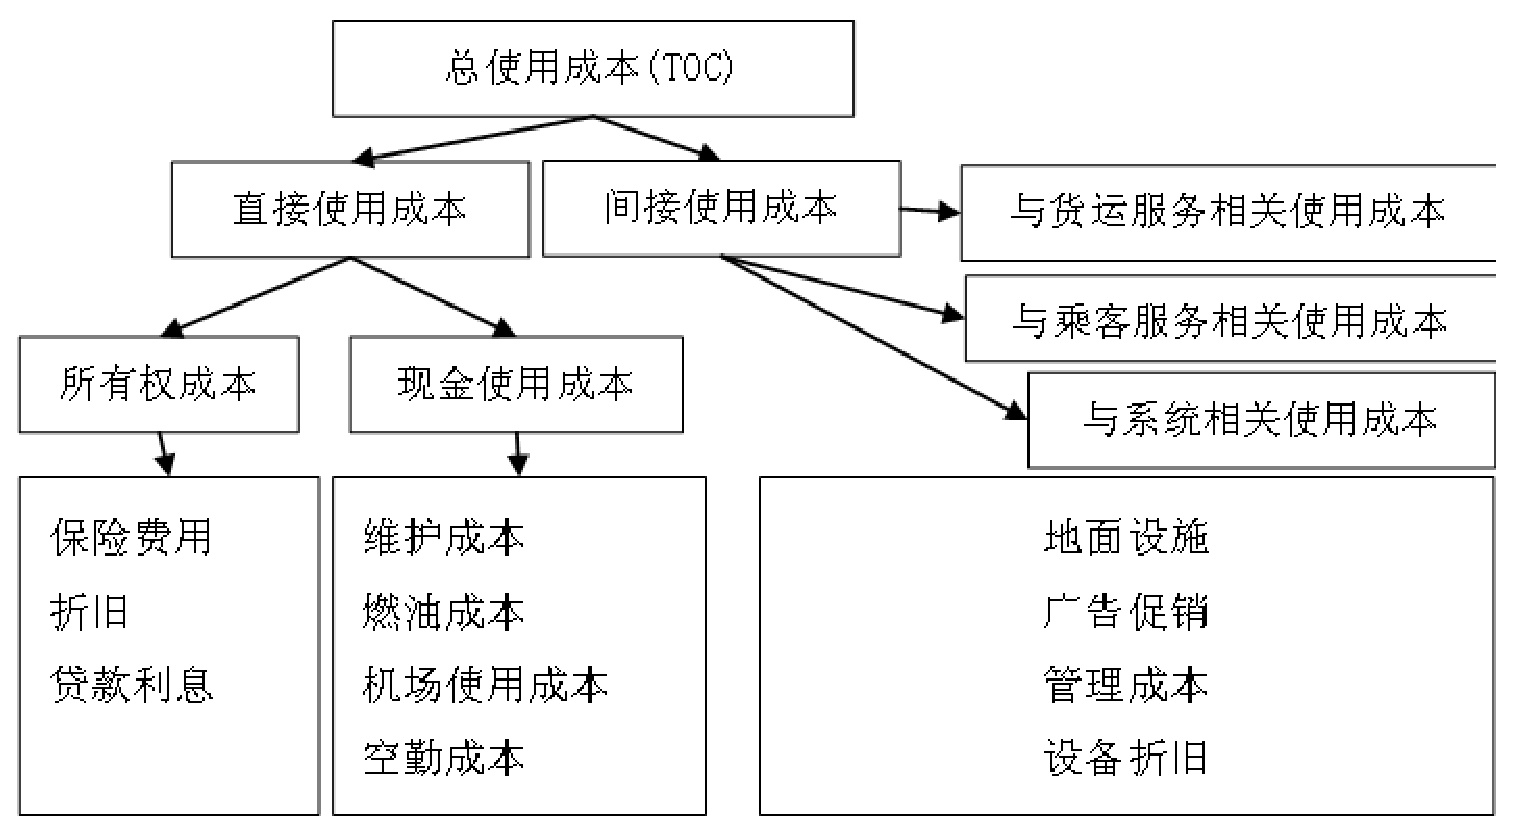
\includegraphics[width=0.8\textwidth]{doc/toc_composition.eps}
  \caption{飞机总的使用经济性(TOC)的构成}
  \label{fig_toc}
\end{center}
\end{figure}

飞机的经济性可以使用下述不同的指标进行衡量,反映飞机直接使用成本的指
标有:
\begin{itemize}
\item[(1)]飞行小时成本(DOC美元/飞行小时)
\item[(2)]航段成本(DOC美元/航段)
\item[(3)]座海里成本(DOC美元/座海里)
\item[(4)]吨海里成本(DOC美元/吨海里)
\end{itemize}
反映飞机制造成本的指标包括:
\begin{itemize}
\item[(1)]单位空机成本(美元/$W_{oe}$)
\item[(2)]单位商载成本(美元/$W_{pl}$)
\end{itemize}

式中,$W_{oe}$和$W_{pl}$分别为使用空机重量(吨)和最大使用商载重量(吨)。其中,最常用的是民机经济性评价指标是座海里成本。

\subsection{经济性评估方法}\label{c13.1.2}
经济性评估可以使用不同的经济性指标进行。准确估算飞机的经济性是一项非常困难的工作,却又是概念设计和初步设计阶段一项非常重要的工作。在这一阶段有关设计方案的数据非常缺乏,众多参数都有待确定。这又为准确估算飞机成本带来了很大的困难。

飞机成本估算的常用方法包括自下而上的方法,从估算零件的成本到整个产品的成本,其中涉及对大量数据的处理,而估算的结果受到多种因素的影响,在概念设计阶段,当许多细节尚未确定时,很难采用这种方法。

第二种方法是基于历史数据进行类比分析来进行估算,这种方法对新飞机研发成本的估算存在很大困难,尤其是当飞机间的技术水平差距较大时,需要采用合适的修正因子。可以利用的方法包括案例推理(Case-Based Reasoning, CBR)以及使用神经网络和模糊逻辑的工具等。

第三种方法通过建立成本与关键设计参数间的关联关系来进行,因而称为“参数法”(Parametric Costing)。将DOC和设计参数进行关联得到的成本模型与重量、性能、几何等模块相集成,进行各种设计参数对经济性影响的灵敏度研究,是目前越来越多采用的方法。

其他在财务分析领域使用的方法包括作业成本法(Activity-Based Costing,ABC)和薄利成本法(Lean Costing),这些方法代表了另一类将成本与资源使用和工程活动进行映射的方法。随着计算建模技术,特别是CAD技术的发展,初步设计阶段可以使用越来越多的详细数据,这一发展趋势使得对部件的制造成本信息的把握越来越准确,尤其是对传统金属类结构形式。多种成本估算方法相结合,能够为初始设计阶段的有效决策提供更多的依据。

\section{飞机经济性分析与计算方法}\label{c13.2}
飞机的经济性,与安全性、舒适性和可靠性一起,是民用客机设计的重要指标。民航市场的激烈竞争,决定了民机经济性的优劣往往对民机项目的成败起着关键的作用。在概念设计和初步设计阶段,需要对竞争机型和不同设计方案的经济性进行分析,尤其是直接使用成本,以便选择合适的参数来达到设计方案的综合最优,提高在市场上取得成功的几率。

市场成功是民机设计经济性指标优劣的重要反映。在考虑经济性的设计过程中,首先应基于对预期目标市场和对航空技术发展水平的分析,对不同方案的成本进行估算,作出对技术选择和方案参数选择的评估,最终完成飞机设计参数的确定。

设计方案对经济性的影响主要体现在以下几个方面,飞机的气动外形参数、结构设计和材料选择将影响飞机的起飞重量和结构可靠性,进而影响到飞机的使用成本。金属结构的飞机设计已经相对成熟,但其能够带来的性能改进也变得有限;提高设计的可靠性,减少维护时间是提高经济性的另一个有效手段,现有维护时间和维护材料成本的估算方法大多是基于金属结构的数据,因此可以应用于目前的估算工作中。燃油成本在飞机的使用成本中占有显著的比重,因此发动机性能,尤其是发动机的燃油效率将直接影响飞机的使用成本;此外,影响飞机使用成本的另一个因素是飞机的全机气动效率。

虽然存在不少经济性分析的模型和工具,但大部分方法和公式都来源于国外的数据和经验公式,不一定完全满足国内的现状,因此需要进行数据和模型的不断修正。采用这些模型和公式计算得出的结果尽管不一定完全准确,但可以用于方案设计阶段进行不同方案经济性的对比。随着方案的进一步细化和数据的不断积累,估算的精确度也会不断提高。

现代民机设计一般采用先进发动机技术,达到增大推力、减少油耗、降低噪声和排放的目的,油耗降低带来燃油成本的降低,可靠性和维修性的改善会降低维修成本。但新技术的研发又提高了发动机的自身成本。在新一代民机中,复合材料的使用超过$50\%$,复合材料具有显著的重量优势,以及良好的可靠性和损伤容限特性,从
而改善了维修间隔时间,降低了维修成本;但由于其制造成本较高而提高了使用成本。此外,电传操纵系统在现代民机中广泛使用,由于需要采用余度技术以确保其可靠性,增加了制造成本。但其对设计的影响,如可以采用放宽静稳定性、载荷抑制、阵风抑制、颤振抑制等功能,又减轻了飞机重量,飞机气动效率的提高减少了燃
油成本。从以上举例可以看出,所有新技术的采用都存在一方面提高研发制造成本,另一方面又降低使用成本的因素。因此需要对可能影响新技术的因素进行综合分析,才能得出最终对经济性的影响结果,从而作出是否使用特定的新技术以及使用的深浅程度的决定。

\subsection{直接使用成本(DOC)}
直接使用成本的计算是一项关键的工作,也是一件困难的工作。从航空工业的发展初期,就将成本的预估和控制作为各个设计阶段的重要内容。早在1944年美国航空运输协会(Air Transport Association of America,ATA)就发表了第一个被广泛接受的直接使用成本的估算方法,之后经过多次改进,并逐步从最早的活塞式发动机扩展到了采用涡轮发动机的飞机上。目前广泛使用的方法就是基于1976年的ATA方法。此外,欧洲也发展了自己的经济性的评估方法,通常称为AEA方法。

各种DOC的估算方法对成本项目的划分基本上是一致的,DOC计算中涉及的成本项目主要包括以下内容:资本成本、机场使用成本、燃油成本、维护成本,以及空勤成本等。各项具体成本项中所包含的具体内容如表\ref{table_docsum}所示。

\begin{table}
\centering \caption{飞机直接使用成本(DOC)的计算元素}
\label{table_docsum}     % Give a unique label
%\begin{tabular}{lp{3.8cm}lp{6cm}}
\begin{tabular}{p{0.20\textwidth}p{0.68\textwidth}}
\hline \hline
资本成本&贷款额度,利率,期限,残值,保险率,寿命期限,配件投资成本等 \\
机场成本&导航服务,降落费用,地面服务,旅客服务,民航基础设施建设基金收费等 \\
机组费用&平均薪资水平,包括飞行员,空乘\\
燃油成本&轮档时间,轮档燃油 \\
维护成本&发动机维护成本,飞机维护成本 \\
\hline \hline
\end{tabular}
\end{table}

民机直接使用成本的计算与飞行任务剖面和飞机的性能直接有关,其中涉及的性能参数包括轮档时间、轮档燃油等。依据飞机设计手册,通常选取的飞行任务剖面如图\ref{fig_flight_profile}所示,其中包含两个部分,第一部分为正常的飞行任务剖面,第二部分为备份燃油航段。其中备用油的规则由以下三个部分组成,包括5\%任务用油,200海里备降转飞用油,和1500英尺高度30分钟待机用油。飞行任务剖面中各航段的燃油计算规则如表\ref{table_fortoc}所示。其中给出的燃油比系数为初步的估计值,或为采用性能计算模块获得的更为准确的数据。

\begin{table}
\centering \caption{DOC计算中轮档燃油的简化计算数据}
\label{table_fortoc}     % Give a unique label
%\begin{tabular}{lp{3.8cm}lp{6cm}}
\begin{tabular}{p{0.08\textwidth}p{0.32\textwidth}p{0.22\textwidth}p{0.18\textwidth}}
\hline \hline 航段 & 描述 & 燃油比($\frac{w_{i+1}}{w_i}$)& 时间(分钟) \\
\hline 1&发动机启动、预热与滑行 &0.98 &7 \\
2&起飞,初始爬升至1500英尺 &0.98 & 计算得出 \\
3&加速,爬升到巡航高度 &0.98 & 计算得出\\
4&巡航 &计算得出&计算得出 \\
5&下降 &0.99 & 计算得出 \\
6&进场与着陆 &0.992& 6\\
7&滑行  &0.99 &7 \\
\hline
8&过失进场 &0.98 & 计算得出\\
9&爬升至20000英尺 &0.98 & 计算得出  \\
10& 20000英尺巡航到备降机场 &计算得出&计算得出 \\
11&下降至1500英尺 &0.99 &计算得出 \\
12&进场与着陆 &0.992& 6\\
\hline \hline
\end{tabular}
\end{table}

\nomenclature{$W_E$}{飞机的运营空重}
在DOC的构成中,各项成本所占的比重都不同,其中最主要的三个构成元素分别为资本成本、燃油成本和维护成本。由于在飞机的采购或租赁中可以采用的财务规则的差异,资本成本的计算存在很多方法,但都与飞机的总投资有关,总投资包括在飞机和发动机上的投资,还包括在配件和地面辅助设备上的投资。在配件和地面辅助设备上的投资通常按照飞机或发动机总价的百分比来确定。在方案设计阶段对飞机机体价格的估算主要是通过关联飞机结构重量和飞机目录价格(list price)近似得到,根据波音的数据可以得到飞机机体的单价估算公式为:
\begin{equation}
\label{eq_boeingprice} P_{tc}=0.0010W_{e}^{0.96}
(\mbox{百万美元},2007\mbox{年})
\end{equation}
式中,$W_e$为飞机的运营空重(单位是lb),图\ref{fig_airplane_price}给出了飞机%
价格与运营空重的经验关系。



\begin{figure}
\begin{center}
  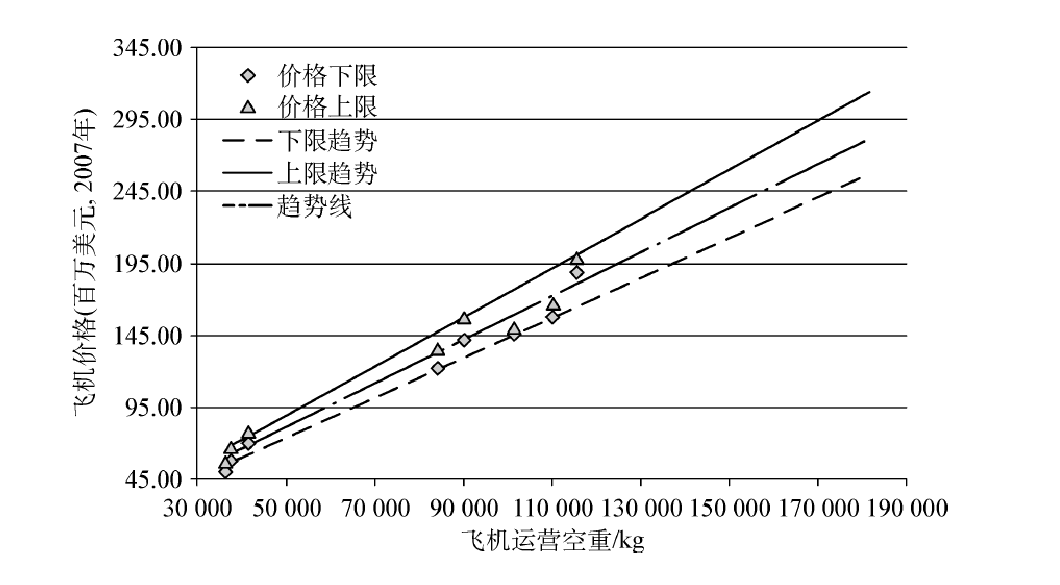
\includegraphics[width=0.8\textwidth]{doc/price_new.eps}
  \caption{飞机机体价格与运营空重间的经验关系}
  \label{fig_airplane_price}
\end{center}
\end{figure}

发动机的价格可以通过关联发动机的推力和燃油效率SFC来得到估算公式为:
\begin{equation}
\label{eq_engineprice}
P_e=1.36×1.5561×[0.3857×(\frac{T_{c}^{0.88}}{SFC^2.58})+0.7286]
(\mbox{百万美元},2007\mbox{年})
\end{equation}
式中,$T_{c}$为发动机的巡航推力(单位为千lbf)。SFC为发动机的燃油效率[单位为lb/(h·lbf)],式中的系数是将货币修正到2007年美元的系数。
\nomenclature{$T_{c}$}{发动机的巡航推力}


飞机的资本成本与资金的来源和使用方式有很大的差别,通常航空公司需要进行详细的评估。一般来说,航空公司可以采用购买和租赁的形式取得飞机的使用权。在这两种形式下,资本成本的计算是不同的,同时还受到各种不同财务制度的影响。

在贷款购买模式下,资本成本的计算是基于飞机机体和发动机的总价来得到的,包括贷款成本、折旧成本和保险成本三个部分。贷款成本的计算可以按如下方式进行,假设贷款总额为$A$,总的还贷次数为$n$,每期还贷利率为$\beta$,每期还款额为$a$,还款年限为$m$,采用等额还本付息方式,每期还款额由以下公式计算
\begin{equation}
a=\frac{A\beta}{1-\frac{1}{(1+\beta)n}}
\label{eq_captitalcost_buy}
\end{equation}
年度利息为
\begin{equation}
i=\frac{n·a-A}{m} \label{eq_captitalcost_interests}
\end{equation}

折旧成本的计算针对飞机机体和发动机的总价格,考虑折旧后的残值和折旧年限用
公式\ref{eq_deprecalc}进行计算。
\begin{equation}
C_d=(P_a+P_e)\frac{1-r}{d_m}
\label{eq_deprecalc}
\end{equation}
式中,$r$是残值所占的百分比,$d_m$为折旧年限。

如果已知飞机和发动机总价,以及保险费率,年度的保险成本计算可以由式%
\ref{eq_doc_insurance}得出
\begin{equation}
\label{eq_doc_insurance} P_{ins}=P_t·r
\end{equation}

机场服务的成本计算将机场服务的成本分解为导航服务费、进近指挥费、航空业务服务费,以及机场地面服务费,与机场服务密切相关的旅客餐食项目也列在此处。导航服务费通常按飞行的里程来计算,进近指挥费根据飞机的降落重量来计算,旅客餐食是根据座舱等级,依据旅客数目进行计算。航空业务服务费和机场地面服务费的计算较为复杂,两者的计算与飞机的设计特点存在一定的联系。

空勤成本在DOC中的计算一般取决于轮档时间,飞机的起飞重量(飞机的种类)和平均单位时间的薪金水平。空乘人员的薪金水平和计算方法因航空公司不同而变化较大,计算中所采用的空乘人员的月薪金水平可以根据我国的平均水平来计算。

燃油成本取决于飞机完成特定航线所消耗的轮档燃油和燃油单价,其中轮档燃油的计算根据典型的任务剖面来进行。计算结果与飞机的性能参数,如巡航速度、巡航时的升阻比,以及发动机的油耗性能之间存在密切的关系。燃油成本在DOC中的比重随着燃油价格的增加而增加,是航空公司运营成本中的重要元素,也反映出改善发动机的油耗特性对改善DOC性能有很大的意义。

维护成本的计算通常分解为飞机维护成本和发动机维护成本,飞机维护成本的计算包括人工成本和材料成本,取决于飞机每年平均的飞行小时、单次任务的飞行时间和飞机的结构重量,在还没有飞机的结构重量估算时,可以采用飞机的运营空重。

在计算DOC的过程中,各种政策性收费,例如我国征收的民航基础设施建设基金也应考虑在内。政策性收费有时是针对特定机型的,比如针对排放严重的老机型等。

\subsection{非直接使用成本(IOC)}
概括来讲,非直接使用成本就是与飞机具体的设计特征没有直接关联的成本项目。这些项目是航空公司开展商业运营活动所必不可少的支出,主要包括下面的一些内容:
\begin{itemize}
\item[(1)]地面设施的所有或租赁,以及使用成本,包括办公室,值机柜台等。
\item[(2)]地面设备成本,包括设备维护,折旧等。
\item[(3)]管理及维护费用。
\item[(4)]总部办公成本。
\item[(5)]广告,销售,以及公关成本。
\item[(6)]票务服务成本,包括订票服务。
\item[(7)]培训成本。
\item[(8)]客户服务成本。
\end{itemize}
非直接成本的计算因航空公司不同而差别很大,作为一个粗略的近似,基于B747%
(四发),DC-10(三发)和两发飞机的统计数据,可以采用如下的公式近似计算%
间接使用成本。
\begin{equation}
IOC=R^{-0.41}[1.19\times{10^{-4}W_{to}}+(0.11+1.17f_1)N_p-3.69](\mbox{百万美元},2007\mbox{年})
\end{equation}
式中,$R$为飞机的任务航程,$W_{to}$为飞机的起飞重量,$f_1$为上座率(乘客数与总座位数之比),$N_p$为总的座位数。从中可以看出,间接使用成本和上座率及飞机的最大起飞重量有关。
\nomenclature{$f_1$}{上座率}

一般来说,设计师对间接使用成本的影响能力是有限的,在设计中需要考虑的主要内容包括地面设备的通用性,以减少购置或租赁新设备的成本,另外,增加驾驶舱设计的共性也有助于降低飞行员的培训成本。

\section{DOC算例}\label{c13.4}
本节以一个具体的民用飞机设计为实例,计算该设计方案的直接使用成本。作为计算实例的是150座级中短程客机,与空客A320和波音B737属于同一个级别,飞机的基本设计参数如表\ref{table_docexample}所示。

\begin{table}
\centering \caption{150座级飞机的基本参数}
\label{table_docexample}     % Give a unique label
%\begin{tabular}{lp{3.8cm}lp{6cm}}
\begin{tabular}{p{0.28\textwidth}p{0.16\textwidth}||p{0.20\textwidth}p{0.16\textwidth}}
\hline \hline 设计参数 & 数值 & 设计参数 & 数值 \\
\hline 最大起飞重量 &73500 kg &发动机型号 &CFM56-5B \\
飞机运营空重 &42175 kg   &发动机台数  &2 \\
载客数  &150 &巡航SFC &0.63 1/hr\\
驾驶员数  &2  &函道比 &5.3 \\
机组人数  &3  &巡航推力   &28.7 kN\\
最大巡航速度   &487 kn  &经济巡航速度  &454 kn\\
\hline \hline
\end{tabular}
\end{table}

在DOC的计算中,假设航段里程为1000 n mile(1852 km),年飞行时间为3000h,计算所用的轮档时间为157min,轮档燃油为6241 kg,由此得出年利用率为1146架次。
根据飞机与发动机的基本参数,人民币汇率采用6.83,可以近似估算出飞机机体和单发发动机的价格如下:

飞机机体价格=$0.00101\times(42175\times2.20462)^{0.96}\times6.83=405.88$百万元

发动机单发价格=$0.5\times1.36\times1.5561\times[0.3857\times(T^{0.88}/SFC^{2.58})+0.7286]=52.65$百万元

飞机的总价为机体价格与两台发动机价格的总和511.18百万元。考虑到飞机配件、发动机配件和地面支持设备的投资额度分别占飞机机体价格、发动机价格和飞机总体价格的百分比分别为8%,20%和1.7%,可以计算得出总投资额为573.40百万元。

如果采用租赁形式,假设租赁保证金比例为10%,租赁期12年,租金为每月支付,年贴现率6%,承租期满的飞机残值为30%,租赁手续费为租金的5%,则每航段租金可以计算为:45333元

假设机长飞行员月薪15000元,副机长飞行员月薪10000元,空乘月薪9000元,其他间接成本占月薪的20%,则计算得出每航段空勤成本为:2717元

每航段燃油成本的计算为:$5.637\times5000=28185$元

民航基础建设基金为:$4259$元

维修成本包括飞机维修成本和发动机维修成本,分别计算为:4408元和2919元,共计7319元。

旅客餐食成本的计算为:$25\times8+16\times142=2472$元

机场服务成本包括如下各项:
导航费与进近指挥费为$0.2\times1852+5\times73.5=737.9$元;机场航空服务收费由于所在机场不同而有所不同,其包括起降费,停场费,客桥费,旅客服务费和安检费,按平均水平计算可以得出:

起降费:$1162.5+23.25\times(73.5-50)=1708.88$元

停场费:$1708.88\times15\%\times365/1146=81.64$元

客桥费:100元(一小时以内)

旅客服务费:$150\times45.75\times0.7=4803.75$元

安检费:$150\times6.25+2\times39.5=1016.5$元

机场地面服务费包括一般代理费,配载/通信/集装设备/旅客及行李服务收费,货物及邮件服务收费,客梯/装卸/地面运输服务,飞机服务和飞机勤务收费,各项收费的计算分别如下:

一般代理费:50元

配载等服务,货物及邮件服务,以及客梯等服务收费:
$16.22\times(33+28+6)=1086.74$元

飞机服务:$120\times2.3=276$元

飞机勤务:$150+160\times0.5\times1.5=270$%

将以上各项收费汇总,可以得出每航段机场服务收费为:9279.23元。

综合上述DOC中的所有元素,可以得出每航段DOC的计算结果为:96212.83元,每座公里DOC为0.35元,每公里DOC为51.95元,每日直接运营成本为302108元。

\section{基于经济性的设计}\label{c13.4}
建立飞机方案的经济性分析模型的目的是通过经济性的分析对比不同设计方案,结合市场分析,研究不同设计参数的影响。基于经济性的设计是指将经济性指标作为飞机参数综合的迭代过程中的目标函数之一,与性能、可靠性、舒适性和安全性等指标同时考虑。

经济性分析对民机设计尤为敏感,是航空公司进行机型选择的出发点和落脚点,因此需要将经济性作为设计流程的有机组成部分进行优化,构建基于经济性的一体化设计体系,如图\ref{fig_economic_design}所示。%
\begin{figure}
\begin{center}
  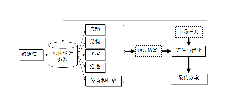
\includegraphics[width=0.8\textwidth]{doc/economic_design.eps}
  \caption{基于经济性的方案设计流程}
  \label{fig_economic_design}
\end{center}
\end{figure}
影响民机经济性指标直接使用成本的主要因素包括飞机的航程,座位数,发动机的油耗等。飞机的性能指标通过轮档时间与轮档燃油影响飞机的直接使用成本,不同设计参数对性能和飞机重量的影响最终反映在飞机的使用成本上面。在建立了飞机的直接使用成本模型以后,可以进行设计参数的灵敏度分析和优化研究。以150座级的飞机设计为例,图\ref{fig_docrange,fig_docseats,fig_docsfc}中分别给出了航程、
座位数和发动机油耗(SFC)对飞机直接使用成本的影响曲线。%
\begin{figure}
\begin{center}
  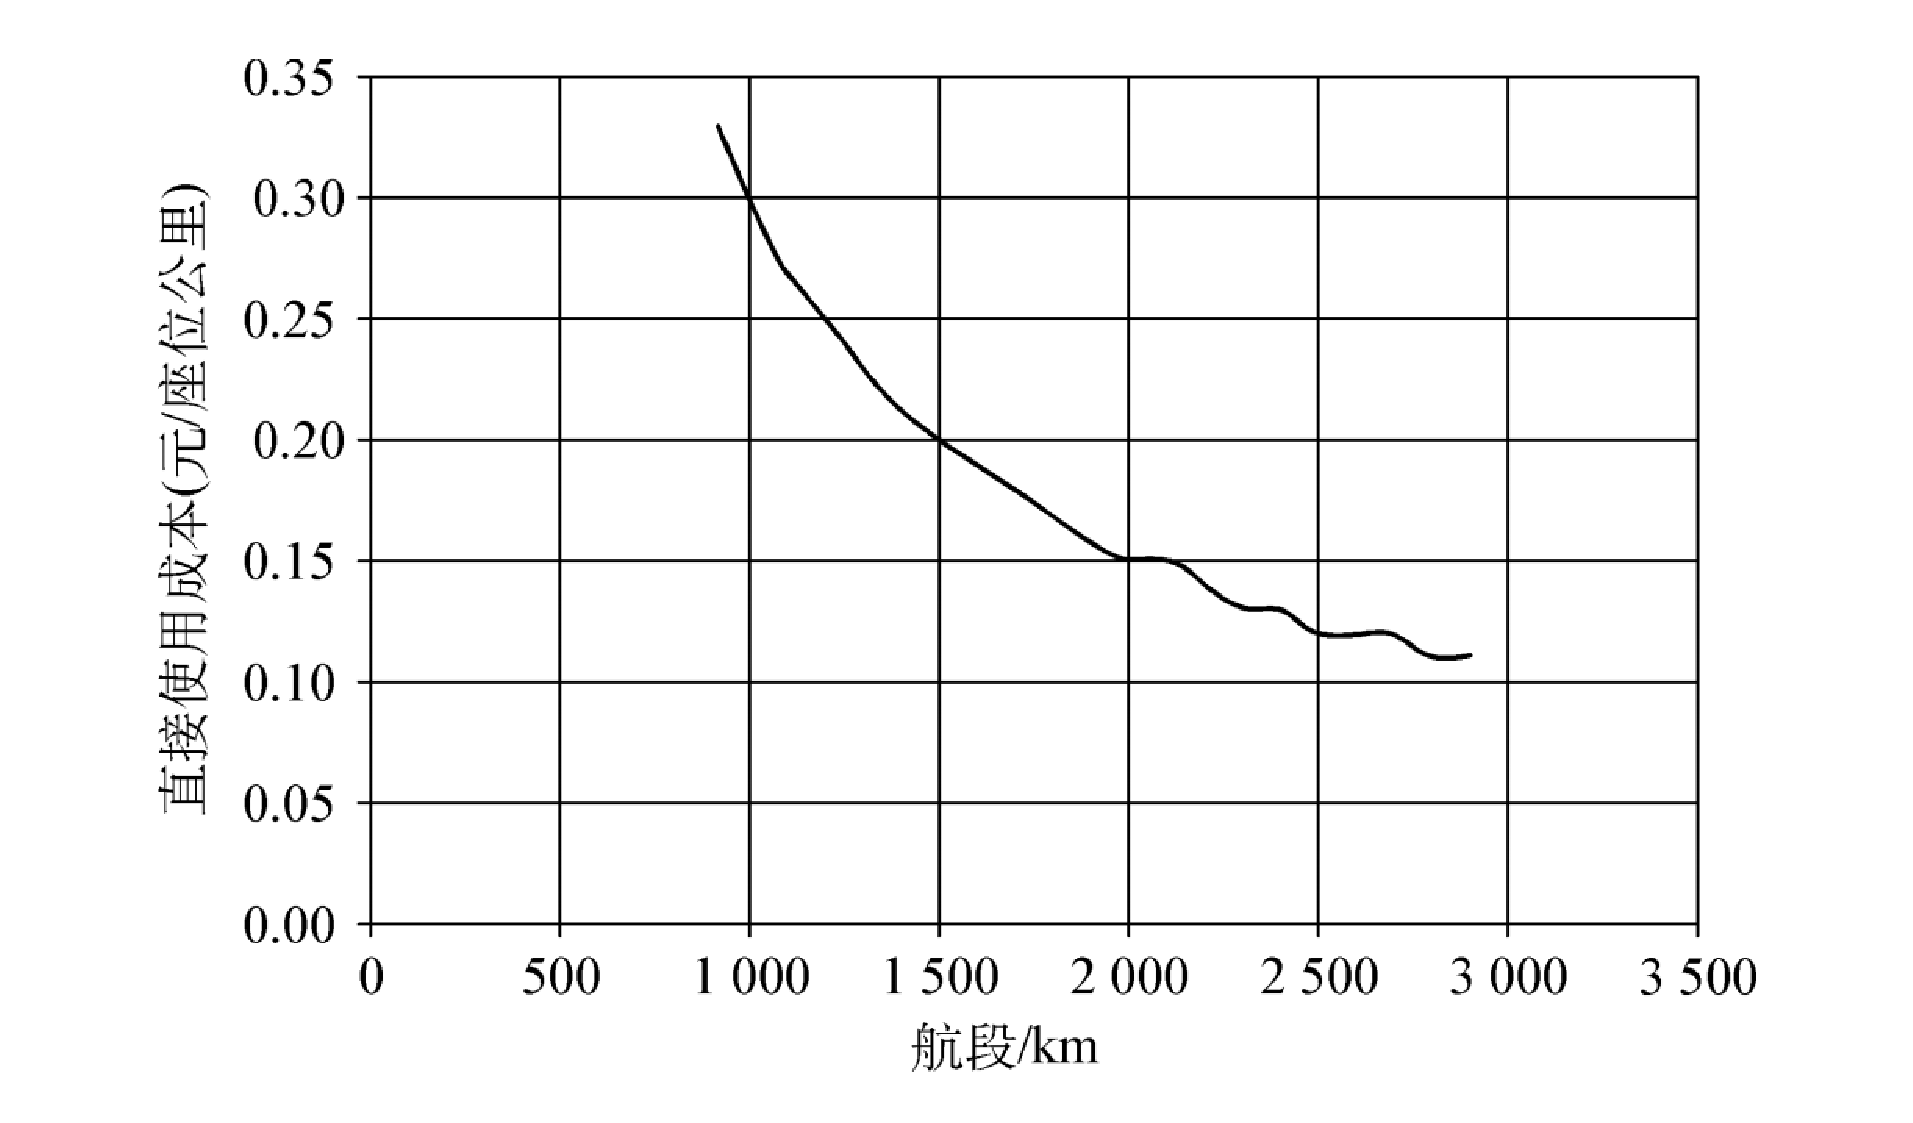
\includegraphics[width=0.8\textwidth]{doc/doc_range.eps}
  \caption{航程对直接使用成本的影响}
  \label{fig_docrange}
\end{center}
\end{figure}
\begin{figure}
\begin{center}
  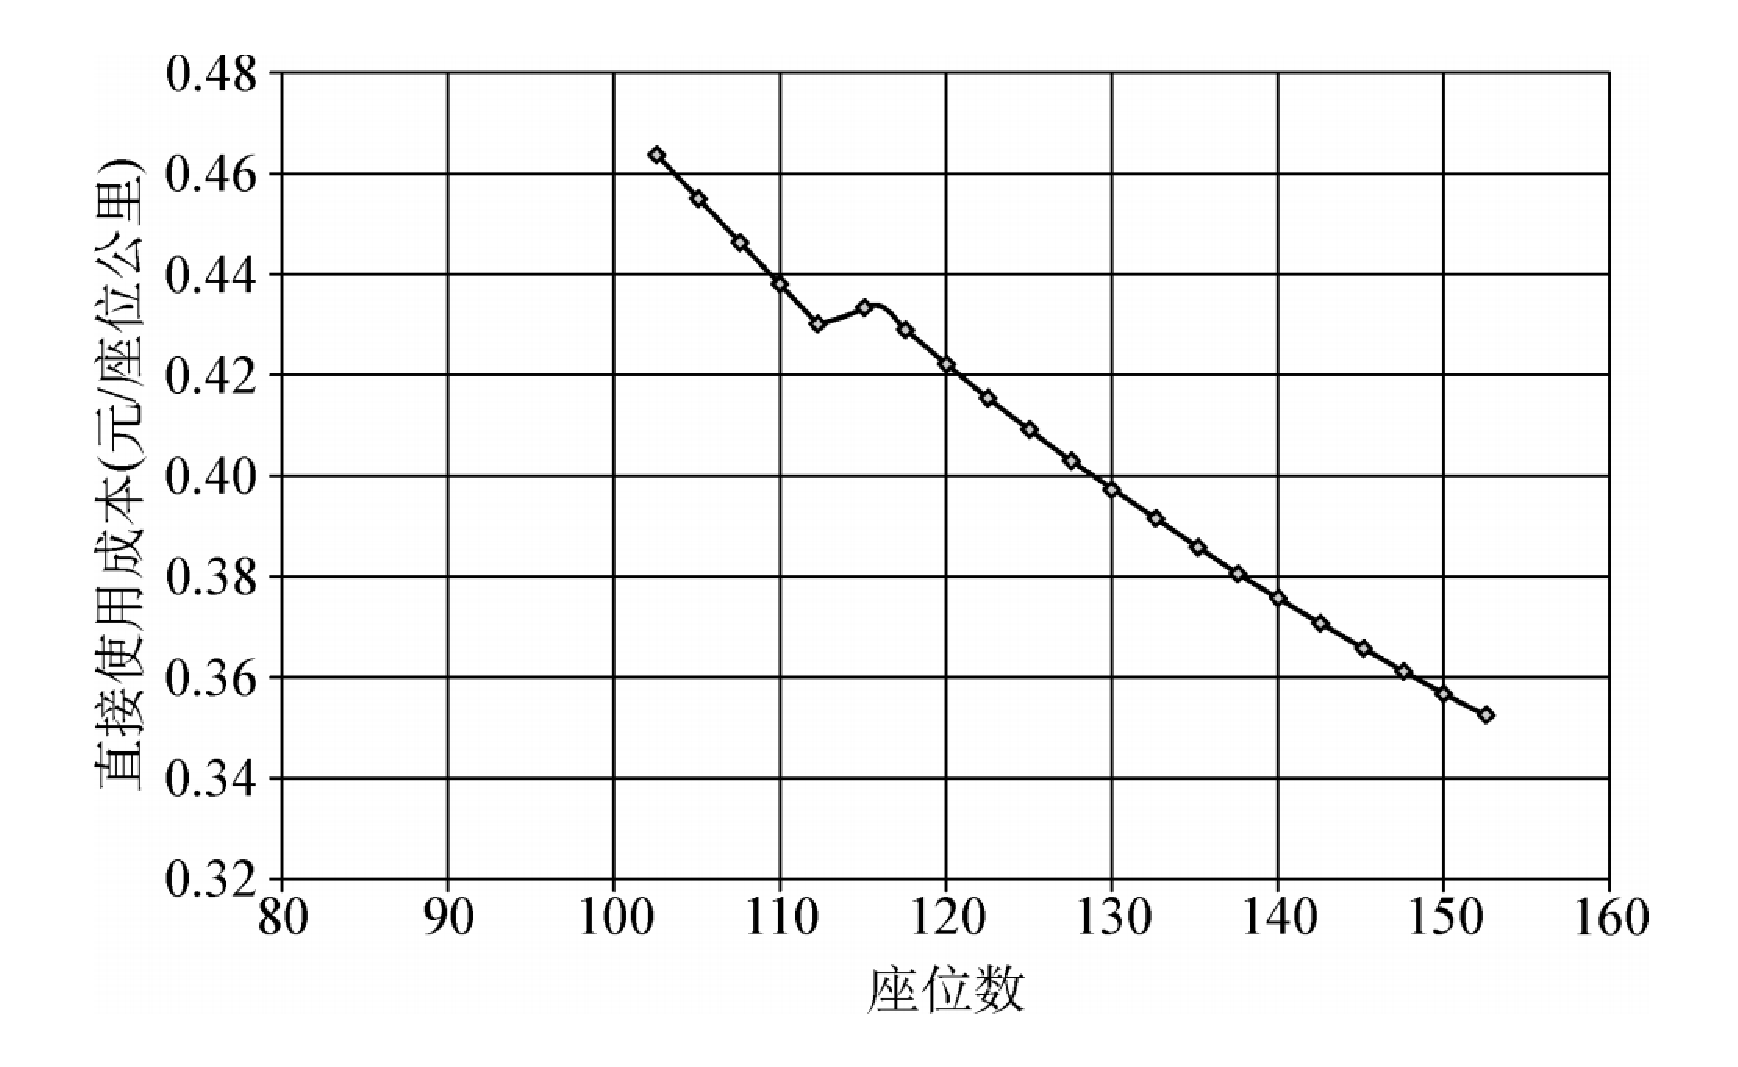
\includegraphics[width=0.8\textwidth]{doc/doc_seats.eps}
  \caption{座位数对直接使用成本的影响}
  \label{fig_docseats}
\end{center}
\end{figure}
\begin{figure}
\begin{center}
  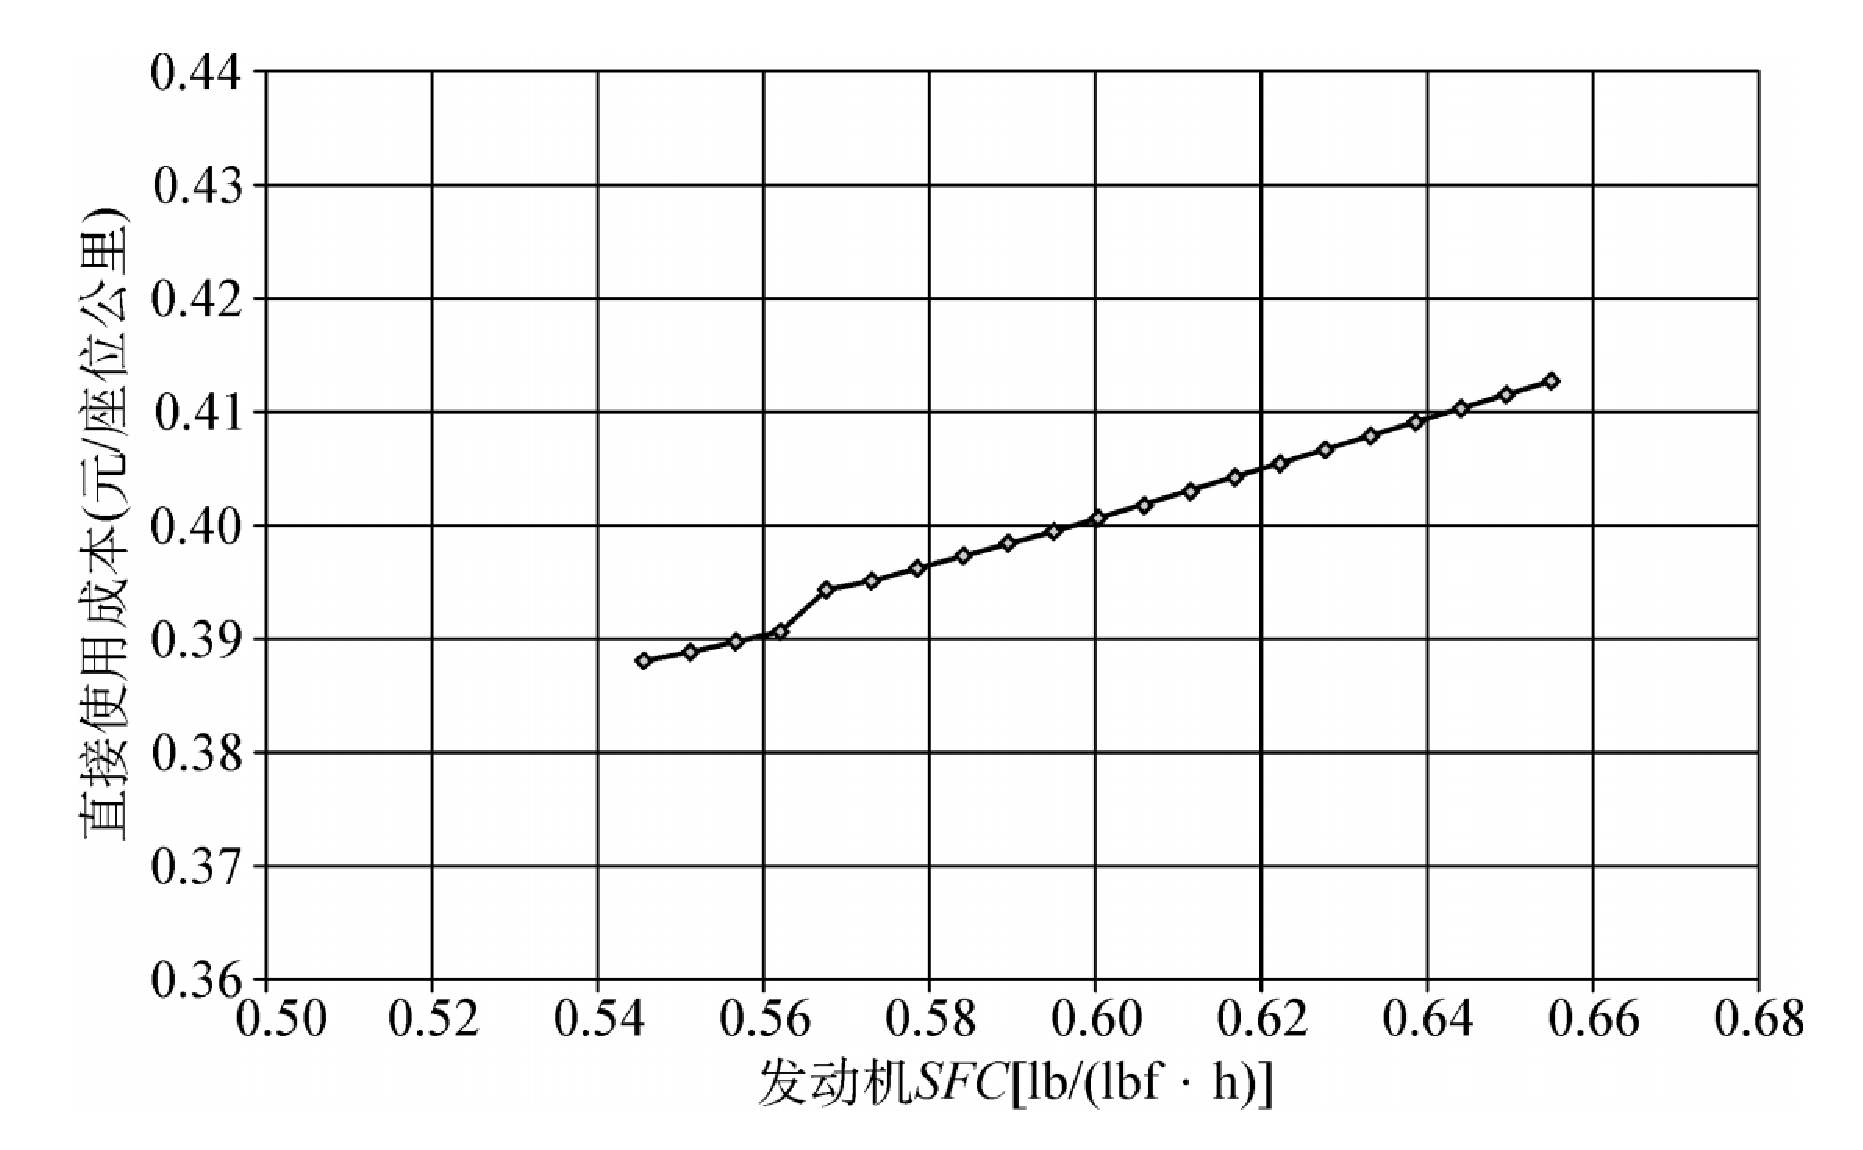
\includegraphics[width=0.8\textwidth]{doc/doc_sfc.eps}
  \caption{发动机油耗SFC对直接使用成本的影响}
  \label{fig_docsfc}
\end{center}
\end{figure}

在有关经济性的设计决策中,应充分考虑所面临的经济环境的不确定性,在设计中利用模糊逻辑等有关的决策工具,以便得出尽可能最优的设计方案。


\chapter{飞机维修成本}\label{ch2}

\section*{引言}


在飞机的长寿命周期中,飞机的维护状态对飞机的性能和价值具有重要的影响。飞机维护成本在飞机使用成本中占重要的比例,是直接使用成本(Direct Operating  Cost,DOC)中的重要成本项,也是全寿命周期成本的组成部分,是关键的飞机的竞争力指标之一。飞机的维修成本和飞机的设计有关,例如系统的复杂性,维护工作的难度体现在所消耗的时间和材料,使用的工具等方面因素。

飞机的维修成本包括飞机机体结构和系统的维护,以及发动机的维护。维护成本的估算在飞机方案设计以及全寿命周期都非常重要,在方案设计阶段对维修成本的考虑将影响不同技术方案的选择,参数的优化,以及对飞机最终的经济竞争力具有长期的影响,在飞机的全寿命周期中,维修成本是实际发生的使用成本的重要部分。

飞机的维护成本受到很多因素的影响,既包括飞机方案设计决策,也包括飞机的使用环境、使用方式,和维护活动。因此,不同机型和不同航空公司的维护成本差异较大,数据的离散度较高,对飞机在使用寿命周期中的价值产生很大的影响,是飞机价值评估中需要考虑的重要因素之一。

对飞机维护成本的估算采用的方法和其他成本项目的估算类似,通过针对维护成本数据与成本驱动因子的关联分析,建立成本估算公式(Cost Estimation Relationship,CER)是常用的方法之一。这种方法的优势在于可以通过成本驱动因子的识别和拟合关系的确立,分析不同影响因素对成本的潜在影响,服务于设计和运营决策。

\section{飞机维护成本}

飞机的维护成本估算包括了直接维护成本(Direct Maintenance Cost, DMC)和管理支出项目,前者和飞机的维护活动直接相关,后者主要取决于航空公司的一些管理方式。大部分的维护成本模型中将两者综合在一起,主要原因在于航空公司在对维护成本的统计汇总将两者并没有明确的分离。直接维护成本(DMC) 的估算存在较大挑战,数据的离散度较大是重要原因之一。

文献\cite{pearlman1966maintenance}中建立了飞机子系统的维护成本的参数模型,其中对成本驱动因子的选择在后续一些针对成本估算的研究中得到广泛使用。文献\cite{fioriti2018cost}中采用IATA的MCTG(Maintenance Cost Technical Group)\cite{mctg}维护成本数据对维护成本的估算公式的驱动因子和拟合得到的估算公式的系数进行了更新。该方法的主要不足在于以下两个方面:

\begin{itemize}
    \item 对于维护成本和驱动因子之间采用了线性假设关系;
    \item 发动机维护成本过于简单,仅仅考虑的发动机数据和发动机推力数据。
\end{itemize}

由于发动机维护成本将是下一节讨论的主要内容,此处重点讨论飞机机体和系统的维护成本的估算方法。这也是主要的维护成本模型中采用的维护成本的分解方法-机体维护成本和发动机维护成本,其中前者包含了结构部件和系统。

在维修成本数据的统计中,一般针对维修活动类型进行,例如航线维修和基地维修,以及部件维修,和发动机维修,其中部件维修一般涉及到的是针对部件和系统供应商开展的维修活动,

典型的维护成本模型包括ATA方法,AEA方法,

在常用的飞机维护成本估算公式

\section{发动机维护成本}


\section{系统维护成本}



\section{小结}

\chapter{飞机经济性设计}\label{design2cost}


经济性指标始终是飞机设计过程中需要考虑的重要因素之一,通过开展项目、产品或服务的技术经济分析,做出最优的决策,一直是实现费效比(Cost-Effective Analysis)提升的关键途径。罗列各种不同的经济性指标:飞机的价格,飞机的研发费用,飞机运营成本,飞机的油耗,飞机运营票价和收入,全寿命成本

\section{飞机经济性设计方法}
采用不同的设计指标可以得到不同的设计方案,这些方案的侧重点不同,使用其他经济性指标进行衡量时就未必能够体系出最优的性能。因此,如何确定最优的设计指标,就成为问题的关键。同时,飞机设计过程中存在的大量技术指标,以及目前越来越受到重视的环保指标,使得问题更加复杂化,需要采用多学科、多目标、多约束的全局和局部相耦合的、多层次的优化方法开展优化设计,服务于决策系统。存在的问题:设计决策的层次化,碎片化;数据量和信息量的增加;决策需求和信息供给失衡问题;对数据的分析方法对经济学、管理学和博弈理论的应用,以及和工程技术领域,信息技术领域的深度融合。

\subsection{基于经济性的飞机总体技术方案设计}
从飞机项目的历史经验来看,在飞机方案设计阶段及初步设计早期的设计决策锁定了飞机全寿命成本的$85\%$以上,也基本决定了飞机的直接使用成本,进而影响了飞机的市场竞争力,因此在设计初期开展不同设计方案以及不同设计参数的经济性分析和优化能够起到事半功倍的效果,也是提高飞机市场竞争力的关键环节。实现分析飞机总体方案中主要技术参数与全寿命周期经济性指标(研发成本、单机成本和直接使用成本等)的关联,提供多技术方案决策时的经济性优化工具。民用飞机经济性设计方法,是将经济性指标作为飞机概念设计综合迭代优化过程中的目标函数之一,与安全性、性能、环保、可靠性、舒适性等指标同时考虑的设计方法。

民用飞机经济性设计的基础在于成本估算,飞机研制中为控制飞机项目的研制成本,降低飞机产品的运营费用,尽管成本的估算方法由来已久,但是需要结合我国制造商实际需求,采用适用的经济性指标。在经济性设计方法中,设计者可以自行通过有机融入到概念设计中的成本模型对设计方案进行经济性评估,并能快速响应设计方案,使设计者能将成本与气动、性能、环保等因素同时考虑。

估算模型的建立,更重要的目的是将成本模型有机融入到概念设计过程中,使得概念设计的设计参数作为成本模型的输入端,提高成本模型对设计参数的敏感性。例如使用飞机的性能数据计算飞行轮挡时间,作为直接运营成本的输入,能很好的增加运营成本对设计参数的敏感性。
为得到经济性良好的设计方案,将经济性分析应用于飞机优化设计过程中,首先需要区分飞机总体设计参数的类型以及其参数范围,例如,对于像飞机的设计航程,飞机座位数,单发升限以及机场的起飞降落距离、进场速度等描述飞机市场适应性的总体设计参数,由于它们是飞机制造商根据目标市场而定的,不需要参与设计迭代。而其他类型的飞机总体方案参数,则是在以经济性指标为目标函数的迭代优化中重点关注的参数。面向经济性的民用飞机总体方案的优化方法的一般流程如下。

首先确定基准机型的总体参数,包括重量、气动和性能等。基准机型应该满足目标市场的设计需求,同时基准机型参数的准确度也很重要,不准确的基准机型参数将会使得总体设计的参数优化产生错误。

随后利用民用飞机经济性设计程序,在满足设计需求的条件下,选择基准机型的几何参数和气动参数(机翼展弦比、机翼面积、机身长细比、增升装置等)、动力参数(发动机推力、发动机单位耗油率等)、设计速度(失速速度等)参数等进行敏感性分析,得出这些总体参数的变化带来的飞机重量、发动机推力需求和轮挡性能等设计参数的变化。
最后,利用经济性估算模型,对参数变化后的设计机型进行经济敏感性分析。以经济性最优为基本原则来选取各项总体设计参数。
在飞机总体方案的设计优化中,以不同的经济性指标为目标函数进行优化都得到了应用,常用的指标包括单机成本,直接使用成本,以及考虑飞机市场价值在内的飞机净现值等,对于商用飞机而言,虽然直接使用成本是客户关心的主要经济性指标,也是飞机设计中的重点考虑的指标,但是,也不能完全忽略其他指标,例如,为了提高飞机的使用经济性而在新技术上的过分投入一方面增加项目风险,另一方面又增加了研发投入,在市场竞争定价的商用飞机市场环境中,大大提高了制造商的财务风险。因此如何平衡制造商和运营商的利益,同时取得市场竞争并非一个简答的问题,需要探索以直接使用成本为主,多种经济性指标相结合的综合应用,以及引入价值链概念,考虑飞机价值随时间动态变化的趋势,综合飞机研制进度影响等内容。这些因素大大增加了飞机概念经济性设计的难度和不确定性。

\subsection{基于经济性的机体结构经济性分析和设计方法研究}
飞机的全寿命周期成本体系中,飞机机体结构的材料和制造成本占据重要的比例,同时还通过影响飞机的重量对飞机的燃油效率和直接使用成本产生影响,随着新材料使用比例的不断增加,如何做出最优的技术经济决策成为一个设计师在飞机总体层次和部件层次面临的问题,需要有效可信的分析方法的支撑。

飞机机体结构的成本估算模型主要包括研发成本和制造成本,服务于飞机全机研制成本和单机成本的估算,对于机体结构部件而言,目前最常用的成本估算方法有三类:工程估算法、参数估算法和类比法,三种方法各有优劣,需要的输入信息量不同,得到结果的准确性也不同。
工程估算法是利用工作包分解自下而上地开展费用估算。由于使用基于物理模型的估算,该方法估算准确度高,但模型涉及的参数众多,信息量大,复杂度高,建模和更改的时间都较长。由于依赖于较多的几何、材料等细节数据,一般该方法都与CAD建模系统紧密融合。

参数估算法是利用汇集起来的用于具有类似用途的飞机的大量现有费用数据,只采用少量的特征参数(如重量、速度等)回归出的一组费用-特征量之间的线性关系式。参数估算法主要应用于项目的初期阶段,在多种方案比较时,能快速及时地为选型决策提供可靠的依据,但是这种方法严重依赖于基础数据的可靠性。需要对数据的长期积累和细致分析。基于参数法和物理仿真模型的费用模型代表了未来发展的方向。
类比法是建立在于过去类似的工程项目进行比较,并根据经验加上修正而得出费用估计。类比法用于旧机改进改型项目估算较为准确,在项目的研制初期,通常作为一种粗略的辅助性方法。

\section{飞机经济性设计体系
}在系统整理飞机的经济性数据的基础上,可以建立完整、灵活的飞机经济性数据体系以及基于飞机经济性分析方法基础上的面向飞机经济性对设计方法以及工具,以满足飞机设计不同阶段的需求,概念设计阶段需要快速并相对准确的经济性指标估算方法,详细设计阶段对成本的估算需要准确可靠,并形成完善的数据积累模式和结果,为经济性设计方法的不断完善提供支撑。
在飞机概念设计阶段对整个项目的经济性影响巨大,需要开展大量设计方案的技术经济性分析;而随着设计的深入,需要处理设计细节对经济性的影响分析,对经济性指标的计算需要达到较高的精度和可靠性;在设计的不同层次,不同的决策人员对项目的决策的影响评估,不同部门的经济性数据的整合、校正、归档和利用也将大大影响整个经济性工作的影响力和可持续性。
可以针对有关的技术数据、经济性数据使用不同的分析方法和结果应用途径


\section{结论}
本报告首先综述目前增升装置CFD分析和设计的主要方法,难点和发展趋势。随后分析了增升装置设计应该遵循的主要原则,设计过程和设计环节中的主要工具的使用。本报告对高效率的增升装置的设计具有一定的参考价值。
\chapter{Value Driven Design}\label{chvdd}

In previous chapters, a number of economic merits have been presented and discussed for its use in the economic evaluation of commercial aircraft and design projects. For example, manufactures tend to use net present value to evaluate the likely break-even point, on the other hand, airlines tend to use direct operating cost in decisions on aircraft purchases. Increase in research and development cost by manufacturers would generally lead to lower operating cost by reducing fuel consumption due to lower aerodynamic drag, structural weight, and lower system maintenance cost etc. When the aircraft sales price is under pressure in a market condition, the manufacturers would face more challenges in achieving financial balances as the increased project could not be passed onto airlines. In market reality, a dynamic balance would be reached, in which, the number of better aircraft would benefit and gradually increase its market share. The total value of the industry is increasing. 

In daily life, we might have different understandings on the concept of value, for example, the value provided a phone has changed from the traditional long-distance talking to video calling and many other applications on the smart phone. The importance of the original functionalities have decreased. This changed the way and merits we evaluate the product changes over time. On the other hand, functionalities provided by other products remained largely the same, but the performance and other aspects simply enhanced its main, original functionality. In both scenarios, the key for sustained success comes from its value creation nature for players from each category along the supply chain. The change in supply chain landscape is undoubtedly driven by fundamentals in the such value creation dynamics. 

Back to aerospace industry, here is a few examples of commercial aircraft development project and defense projects. The focus is on the economic performance. There is no doubt that the reasons for such delays and over budget are very complex including technical challenges, policies, economic conditions, management, etc. Due to its important impact on the project, company and sometimes on the health of the whole industry, significant effort have been devoted to this challenge. Value-driven design is one such methodology. 








\chapter{Aerospace Supply Chain}\label{ch-supply}

Just as in any other industry, supply chain and its management is a critical issue and a reflection of the industrial competitiveness. The aerospace supply chain has its unique features such as its multi-tier structure, strong integration of defense sector and civil business, high barriers of entry, high demand for capital and technology, etc. Aerospace supply chain is also strongly affected by factors of geopolitics.

The status of aerospace supply chain has evolved over the last four decades due to globalization and outsourcing, rapid development of Chinese economy and industrial capabilities. The fundamental driving factor for supply chain evolution is the transfer of value creation activities. Such transfer maybe prompted by factors such as low cost manufacturing, closer to market, tax or tariff avoidance. 

\section{Introduction}
Design, development, manufacturing, and after-sale services often involves large number of different companies and partners in either a simple or a complicated process of information and physical flows.  Commercial off-the shelf (COTS) or commercially available off-the-shelf products are packaged solutions which can then be adapted to satisfy the needs of the purchasing organization, or integrated into a bigger system, rather than the commissioning of custom-made, or bespoke, solutions. COTS provides alternative to custom-made solutions in terms of lower cost and wider availability. 


\section{Concept of Supply Chain and its Management}




It can be expected that the performances of different suppliers are different, the question here is what are the possible criteria that can be used in the choice and evaluation of suppliers. 



\section{Aerospace Supply Chain}
Over the last hundred years, and the last four decades in particular, the aerospace industry has evolved greatly. Such changes can be found in technology base, business models, design methods and tools. 



\cleardoublepage
\printbibliography[title=参考文献]
%\printbibliography[heading=bibintoc,title=参考文献]

\end{document}
